\chapter{Project Analysis}\label{ch:project-analysis}

\section{Stakeholder Analysis}\label{sec:stakeholders-analysis}
Developing a platform like Chronocademy required a strong awareness of the various stakeholders involved.
Recognizing and categorizing these stakeholders provided the team with a clearer understanding of the platform’s purpose, requirements hierarchy, and potential challenges.
By addressing these three core aspects, the team ensured a professional and structured approach to project development.

For clarity, we define a stakeholder as:

\begin{quote}
``A person or group of people who own a share in a business or a person such as an employee, customer, or citizen who is involved with an organization, society, etc.\ and therefore has responsibilities towards it and an interest in its success.'' \cite[Stakeholders]{stakeholder}
\end{quote}

In this section, the reader will find a list of all the potential stakeholders, should this business succeed:

\begin{itemize}
\item Learners (Primary Users): Individuals looking to acquire new skills but constrained by financial barriers.
They are the primary audience, relying on the platform to find suitable courses and teachers.
\item Teachers (Primary Users): Individuals with expertise in specific skills who want to share their knowledge.
They use the platform to offer lessons and earn time credits, motivating them to participate actively.
\item Platform Administrators (Internal Stakeholders): The team responsible for maintaining, managing, and improving the platform.
They ensure smooth operations, manage user accounts, and resolve technical issues.
\item Developers (Internal Stakeholders): The technical team responsible for building, deploying, and maintaining the Chronocademy application.
Their role is crucial for implementing features and ensuring performance and security.
\item Investors/Sponsors (External Stakeholders): Individuals or organizations that fund the platform’s development or support its long-term goals.
Their interest lies in the platform’s growth, user base, and potential returns.
\item Educational Institutions (External Stakeholders): Schools, training centers, or non-profit organizations that might collaborate with the platform to offer courses or expand their reach.
\item Community Members (Indirect Stakeholders): Families, friends, or networks of users who may indirectly benefit from the platform by accessing shared skills or recommendations.
\item Hosting and Service Providers (External Stakeholders): Companies like Fly.io or other infrastructure providers that support the hosting, storage, and scalability of the platform.
Their stability and reliability directly impact Chronocademy’s performance.
\item Regulatory Bodies (External Stakeholders): Authorities ensuring that the platform complies with local laws, including data protection, financial transactions, and online education standards.
\end{itemize}

\subsection{Stakeholder Identification}\label{subsec:stakeholders-identification}
After recognizing all the involved parties and categorizing them as stakeholders, a power-interest matrix was created to group them by their level of influence and interest.
This tool helped us to understand how to address each group during our project development.

\begin{figure}[h]
    \centering
    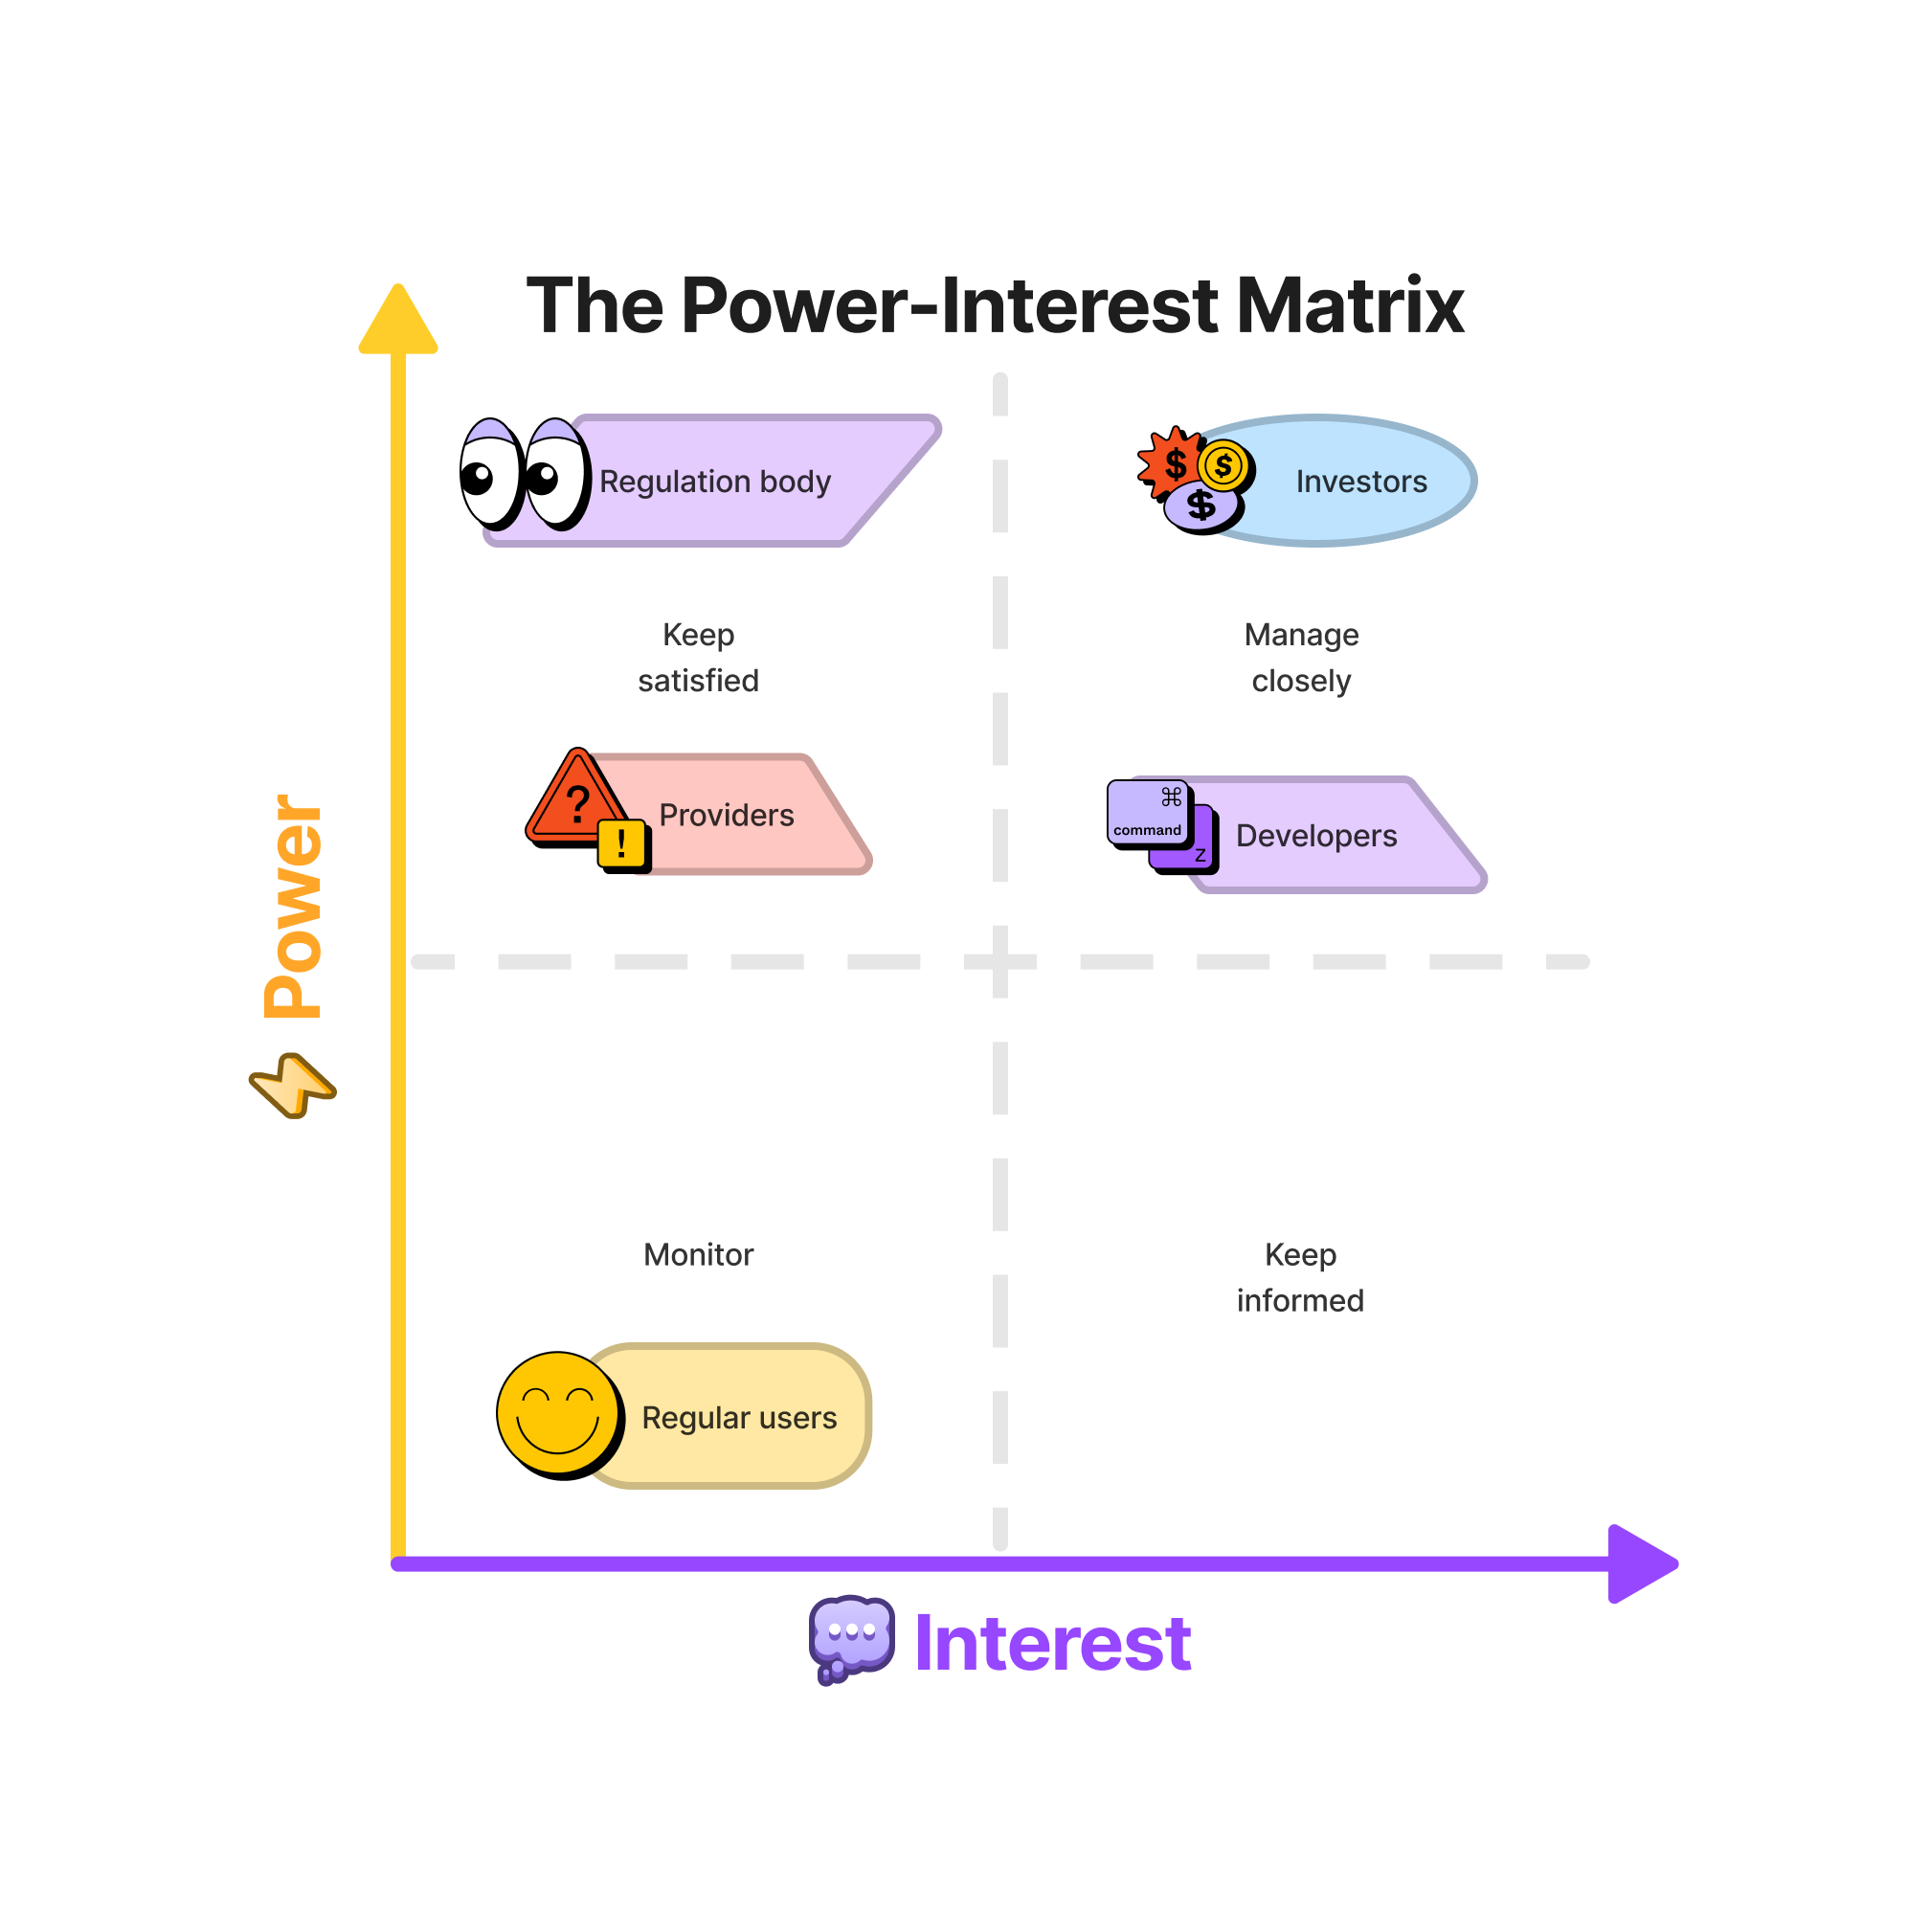
\includegraphics[width=12cm]{stakeholder-matrix}
    \caption{Stakeholder Matrix}
    \label{fig:figure0}
\end{figure}

\subsubsection*{1. Keep Satisfied (High Power, Low Interest):}
\begin{itemize}
\item Regulatory Bodies: Ensure compliance with laws and regulations; their approval is crucial but their active interest is low.
\item Hosting and Service Providers: Provide infrastructure reliability; influence platform uptime but have limited engagement with the project.
\end{itemize}

\subsubsection*{1. Manage Closely (High Power, High Interest):}
\begin{itemize}
\item Investors/Sponsors: Fund the platform and influence its strategic direction.
\item Developers: Build and maintain the system; essential for success.
\end{itemize}

\subsubsection*{3. Monitor (Low Power, Low Interest):}
\begin{itemize}
\item Community Members: Indirectly impacted by the platform; limited influence and occasional involvement.
\end{itemize}

\subsubsection*{4. Keep Informed (Low Power, High Interest):}
\begin{itemize}
\item Learners (Primary Users): Highly engaged users eager to access educational resources.\ Their satisfaction and feedback shape the platform’s usability.
\item Teachers (Primary Users): Key contributors interested in sharing their skills and engaging with the system.
\end{itemize}

\section{Problem Analysis}\label{sec:problem-analisys}

\subsection{Problem}\label{subsec:problem}
Today, many people want to learn new skills, but financial constraints often make this difficult.
Traditional learning platforms require users to pay upfront, which can be a barrier for those who cannot afford the costs.
On the other side, there are many skilled individuals who want to share their knowledge but don’t have a good way to earn money or gain recognition for their teaching.
This situation creates an imbalance, where learning and teaching opportunities are not equally available to everyone.

\subsection{Solution}\label{subsec:solution}
Chronocademy is designed to solve this problem by introducing a platform that
uses a time-based currency called Chrono.
With Chronocademy, users don’t need money to learn or teach skills.
Instead, they can earn Chronos by teaching classes on topics they are skilled at, like computer science, languages, or even cooking.
These earned Chronos can then be spent to book lessons and learn new
skills from other users.
For added flexibility, users who need more Chronos can purchase them with real money, and teachers can even convert their earned
Chronos into cash if they choose to.
This creates a fair and flexible system
that works for both learners and teachers.

The platform also makes the process of learning and teaching easier by integrating tools like Google Calendar for scheduling and Google Meet for video sessions.
These features allow users to focus on learning and teaching, without the hassle of juggling multiple apps for scheduling, communication, or payments.

Chronocademy includes several features to make it an engaging platform for its
users.
People can exchange a wide variety of skills, from practical ones like
cooking to technical ones like coding.
A review system ensures that the quality of classes remains high, so users can trust the lessons they book.
The platform also offers new users free Chronos as a welcome bonus, so
they can start learning right away.
To grow the community further,
Chronocademy includes a referral program where users earn extra Chronos by
inviting their friends to join.

Chronocademy stands out because it removes the need for money in learning and teaching, making education more accessible to everyone.
It also creates a community of people who are motivated to share knowledge and grow together.
By providing a simple, fair, and user-friendly experience, Chronocademy offers an innovative way to connect learners and teachers while making education available to as many people as possible.